%!TEX root = ../thesis.tex
%2-Tools for spectral analysis
% Reduction processes for NIR
% Additions to IRAF toolchain
% Problem with order tracing
%
% Wavelength Calibration
%    All detectors together
%    With stellar and ThAr lines???
% Telluric Correction


\chapter{Tools for spectral analysis}  % Main chapter title
\label{cha:reduction} 

%----------------------------------------------------------------------------------------
%	SECTION 1
%----------------------------------------------------------------------------------------
The work of this thesis relies on the use of NIR spectra obtained by the CRIRES instrument. This chapter contains an overview of NIR reductions steps undertaken, a comparison of model used and post reduction steps taken to make the spectra usable for the follow chapters.  

\section{NIR spectroscopy}
Specifics of NIR verse optical


- dark current
The dark current is due to the thermal motion of elections in the detector


\subsection{Output files}
Main Extraction components
\subsubsection{Dark current}

As the dark current depends on the exposure time there a multiple dark current files. 
These are averaged together and subtracted from the observed science frames. 

\missingfigure{Dark current image for 3 seconds and 180 seconds.}


\subsection{Flat field}
Correct for no-uniform illumination and non-linearity

The dark current created for the same time as the flats is used.
These are average together.


Non -linearity calibrations


\subsection{Lamp files}
Wavelength calibration
We apply wavelength calibration below

Observed output




We explored two different extraction pipelines. The ESO CRIRES pipeline and a in-house pipeline originally used in \citet{figueira_radial_2010} called DRACS (Data Reduction Algorithm for Crires Spectra) .

The spectra were initially reduced using the ESO CRIRES pipeline \href{ESO CRIRES pipeline}{ESO CRIRES pipeline}, with the\href{https://www.eso.org/sci/software/gasgano.html}{GASGANO} interface.  CRIRES pipeline user manual 

%-----------------------------------
%	SUBSECTION 1
%-----------------------------------
\subsection{Subsection}


%-----------------------------------
%	SUBSECTION 2
%-----------------------------------

\subsection{Subsection 2}
Useful information about MIR reduction in the 
\href{https://www.eso.org/sci/facilities/paranal/instruments/visir/doc/VLT-MAN-ESO-14300-3514_2018-02-01.pdf}{VISIR manual}
%
%----------------------------------------------------------------------------------------
%	SECTION 2
%----------------------------------------------------------------------------------------

\section{Main Section 2}

NIR Data reduction:
Extensive effort was made to reduce these spectra, comparing two different techniques.
- corrections
- NIR reduction stages.
- spectral artifacts
- correction of artifacts
Crires reduction
- ESO gasgano
- DRACS
- Post dracs stages
- hindsight 



\subsection{CRIRES data}
\label{subsec:CRIRES} 
Observations were performed with the CRIRES instrument~\citep{kaeufl_crires_2004} configured to observe a narrow wavelength domain of the K-band between 2120--2160~nm using the Ks and the Hx5e-2 filters. The slit width of \(0.4\sec \) resulted in an instrumental resolving power of \(\rm R=50\,000\), with no adaptive optics to ensure that the slit was entirely covered by each target. This prevents strong slit illumination variations that could change the shape of spectral lines.

The observations were performed in service mode during period 89 with run ID.~089.C-0977(A) between April and August 2012. An observation is composed of 8 individual spectra with an integration time of 180 seconds, observed in the ABBAABBA nod cycle pattern to obtain a high (>100) signal-to-noise when combined. The list of observations obtained with CRIRES are provided in Table~\ref{tab:observations}.

\begin{table*}
	\centering    
	\caption{Details about the CRIRES observations times and settings. The estimated RV values for both component in each observation are provided. These are calculated using the best known orbital parameters and the companion mass \((M_{2}\sin{i}/M_{2})\). For hosts with multiple companions the RV value is for the largest companion only i.e. \object{HD 202206}B and \object{HD 168443}c. The RV difference between the host and the companion (\(RV_2 - RV_1\)) corresponds to the \(rv_2\) parameter in the binary model from Sect.~\ref{subsubsec:binary-model}.}
	\begin{tabular}{l c c c c r@{.}l r@{.}l r@{.}l}
		\toprule
		Object & Obs. \# & Start date  & Filter & Airmass  & \multicolumn{2}{c}{\(RV_1\)} & \multicolumn{2}{c}{\(RV_2\)} & \multicolumn{2}{c}{\(rv_2\)}  \\  % & \(Date \)
		&   & (yyyy-mm-dd hh:mm:ss)  &  & (at start) & \multicolumn{2}{c}{kms\(^{-1}\)} & \multicolumn{2}{c}{kms\(^{-1}\)} & \multicolumn{2}{c}{kms\(^{-1}\)}\\ % data ref    % & (JD\(^{\star} \))
		\midrule
		\object{HD 4747}   & 1 & 2012-07-06 07:36:06 & Ks     	      & 1.25  	  & $-$0    & 219 & $-$0  & 154 & 0&065 \\ %-1      & 2456114.81674
		\object{HD 162020} & 1 & 2012-07-04 06:23:22 & Ks     		& 1.30 		& $-$28  & 760 & 50 & 785\tablefootmark{a} & 79&545\tablefootmark{a} \\ %-1      & 2456112.76624
		\object{HD 162020} & 2 & 2012-07-04 06:57:48 & Ks     		& 1.44  	& $-$28  & 717 & 48 & 440\tablefootmark{a} & 77&157\tablefootmark{a} \\ %-2      & 2456112.79015
		\object{HD 167665} & 1 & 2012-07-28 05:00:53 & Hx5e-2 	& 1.24 		& 7         & 581 & 18 & 024\tablefootmark{a} & 10&443\tablefootmark{a} \\ %-1a     & 2456136.70895
		\object{HD 167665} & 2 & 2012-07-28 05:37:27 & Hx5e-2 	& 1.39  	& 7         & 581 & 18 & 025\tablefootmark{a}  & 10&444\tablefootmark{a} \\ %-1b     & 2456136.73434
		\object{HD 167665} & 3 & 2012-08-05 02:54:03 & Hx5e-2 	& 1.04  	& 7         & 575 & 18 & 163\tablefootmark{a} & 10&588\tablefootmark{a} \\ %-2      & 2456144.62087
		\object{HD 168443} & 1 & 2012-08-05 04:29:32 & Ks     		& 1.31 		& $-$0   & 121 & 50 & 932\tablefootmark{a, b}  & 51&053\tablefootmark{a,b} \\ %-1      & 2456144.68718
		\object{HD 168443} & 2 & 2012-08-05 04:58:50 & Ks     		& 1.47 		& $-$0   & 121 & 51 & 189 \tablefootmark{a, b} & 51&310\tablefootmark{a,b} \\ %-2      & 2456144.70753
		\object{HD 202206} & 1 & 2012-07-12 06:54:44 & Ks     		& 1.01 		& 14      & 843 & 12 & 992\tablefootmark{b}  & -1&851 \\ %-1      & 2456120.78801
		\object{HD 202206} & 2 & 2012-07-13 05:41:40 & J       		  & 1.01 	  & 14      & 837 & 13 & 065\tablefootmark{b}  & -1&772 \\ %-2      & 2456121.73727
		\object{HD 202206} & 3 & 2012-07-11 08:29:55 & Ks     		& 1.15		& 14      & 849 & 12 & 920\tablefootmark{b}  & -1&929 \\ %-3      & 2456119.85411
		\object{HD 211847} & 1 & 2012-07-06 07:02:57 & Ks     		& 1.07 		& 6        & 613 & 7   & 171 & 0& 558\\ %-1      & 2456114.79372
		\object{HD 211847} & 2 & 2012-07-13 06:54:37 & Ks     		& 1.05 		& 6        & 614 & 7   & 167 & 0&553 \\ %-2      & 2456121.78793
		\object{HD 30501}  & 1 & 2012-04-07 00:08:29 & Hx5e-2 	 & 1.60 	 & 22      &  372 & 36 & 377 & 14&005 \\ %-1      & 2456024.50590
		\object{HD 30501}  & 2 & 2012-08-01 09:17:30 & Hx5e-2    & 1.42		 & 22      & 505 & 35  & 120 & 12&615 \\ %-2a     & 2456140.88716
		\object{HD 30501}  & 3 & 2012-08-02 08:47:30 & Hx5e-2 	 & 1.53 	 & 22      & 507 &  35 & 102 & 12&595 \\ %-3      & 2456141.86633
		\object{HD 30501}  & 4 & 2012-08-06 09:42:07 & Ks     		 & 1.28 	 & 22      & 514 & 35 & 031 & 12&517 \\ %-2b     & 2456145.90426
		\bottomrule
		
	\end{tabular}
	\tablefoot{
		\tablefoottext{a}{Maximum RV given \(\textrm{M}_2\sin{i}\) only.}
		\tablefoottext{b}{Largest mass companion only.}
	}
	\label{tab:observations}
\end{table*}


\subsubsection{Data reduction}
\label{subsubsec:reduction}
The observations were reduced using a custom reduction pipeline \citep{figueira_radial_2010} with some of the parameters altered to better suit the K-band instead of the H-band setting it was originally designed for. Written in IRAF's CL\footnote{IRAF is distributed by the National Optical Astronomy Observatories, which are operated by the Association of Universities for Research in Astronomy, {Inc.}, under cooperative agreement with the National Science Foundation.} \citep{tody_iraf_1993} it provides for automated dark and non-linearity corrections (using the non-linearity coefficients provided by ESO), as well as the flagging and replacement of bad pixels. The images were corrected from sensitivity variations by dividing by a flat-field corrected from the blaze function effect. The nodding pairs were mutually subtracted and the order tracing was fitted by cubic splines.  

There are two types of extraction commonly used. The \emph{rectangular} extraction performs a rectangular aperture sum in the spatial direction while the \emph{optimal} extraction \citep{horne_optimal_1986} also includes variance weighting to reduce the impact of the noise and deviant pixels on the total flux measurement. Each extracted nod-cycle spectrum is then normalized by dividing by a polynomial fitted to the continuum, with the degree selected for each spectrum and detector.

At this point one would normally combine all the nod spectra together to improve the signal. However, we found that for some spectra the presence of cosmic rays or bad pixels heavily affected the variance weighting during the \emph{optimal} extraction. This caused noticeable extended artifacts in the extracted spectra of individual nods. An example of this can be seen in Fig.~\ref{fig:nod_artifacts}. This created flux deviations in the combined optimally extracted spectra of \(\sim 0.5\% \).  Therefore, we took measures to remove these artifacts before combining the nod spectra as we are trying to recover companion spectra with expected flux ratios \(\rm {F_2}/{F_1} < 1\% \). 

The individual nod spectra that contained artifacts were visually identified by comparing all 8 nod spectra together, as shown in Fig.~\ref{fig:nod_artifacts}, and also inspecting the difference between the mean and the median of the 8 nod spectra. The optimally extracted nods that contained artifacts (top panel) were replaced with their rectangularly extracted counter-parts (middle panel). An iterative 4-\(\sigma \) rejection algorithm\footnote{Found at \url{https://github.com/jason-neal/nod_combination}} was applied to the replacement rectangular extractions to remove the erroneous pixels that caused the artifacts. The \(\sigma\) value for each pixel was calculated as the standard deviation of the nearest 2 pixels on either side of all 8 nod spectra. The rejected pixels were replaced using linear interpolation.

For the remainder of the paper we use combined spectra constructed by averaging the 8 nod-cycle spectra together, where some of the optimally extracted spectra have been replaced using the above method. The last panel of Fig.~\ref{fig:nod_artifacts} shows that the difference between the combined optimally extracted spectra and the \emph{combined extraction with replacements}.

\missingfigure{Example of an artifact in the optimally extracted spectra. The top panel contains the 8 normalized nod spectra after optimal extraction, while the middle panel shows the rectangular extraction for the exact same spectra. A vertical offset is included between each spectra. A single large spike in the seventh nod (pink) near pixel 230 creates a wide and noticeable artifact in the optimal extraction. The bottom panel shows the difference between a combined spectrum using the optimal nods only and a combined spectrum in which the seventh nod is replaced with its rectangular counterpart. The nod spectra are in observation order from top to bottom.}
% \begin{figure}
% 	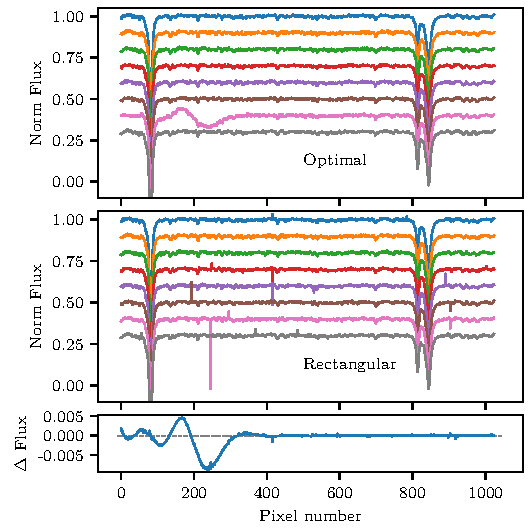
\includegraphics[width=\hsize]{images/final/Bad_pixel_replacement.pdf}  % chktex 8
% 	\caption{Example of an artifact in the optimally extracted spectra. The top panel contains the 8 normalized nod spectra after optimal extraction, while the middle panel shows the rectangular extraction for the exact same spectra. A vertical offset is included between each spectra. A single large spike in the seventh nod (pink) near pixel 230 creates a wide and noticeable artifact in the optimal extraction. The bottom panel shows the difference between a combined spectrum using the optimal nods only and a combined spectrum in which the seventh nod is replaced with its rectangular counterpart. The nod spectra are in observation order from top to bottom.}
% 	\label{fig:nod_artifacts}
% \end{figure}

The normalization and nod combining steps were also performed using IRAF while the following post reduction procedures and analysis all utilize \emph{Python}. This pipeline was chosen over the ESO CRIRES pipeline because it seemed relatively simple to use, being mostly automated, and appeared to have less bad pixel/cosmic ray artifacts in the resulting spectra. In hindsight this was not the case, with artifacts appearing that needed to be removed. 

One possible explanation for the artifacts present is an instrumental effect, such as instrument glow. This is known to affect CRIRES and included in the data reduction cookbook \citep{smoker_very_2012}. These artifacts in the K-band spectra were not observed in previous works in the H-band using this pipeline and as such may have a wavelength dependent affect, as the higher wavelength nIR is more susceptible to thermal instrument glow.


\subsubsection{Wavelength calibration}
\label{subsec:wave_cal}
There is a known issue with the wavelength calibration from the CRIRES Th-Ar calibrations \citep{kerber_laboratory_2009}, due to the low density of Th-AR lines in the near-infrared and the alignment with the detectors narrow wavelength range (e.g.\ CRIRES-POP \citep{nicholls_crirespop_2017}).
Therefore, we use the telluric absorption lines present in each observation as the wavelength reference. Instead of directly using the HITRAN database \citep{rothman_hitran2012_2013} for the line positions of the telluric spectra (e.g.~\citep{brogi_signature_2012,brogi_carbon_2014,dekok_detection_2013}), we use TAPAS atmospheric transmission models \citep{bertaux_tapas_2014} obtained for each observation. These in turn use the HITRAN database but include atmospheric profiles and physical measurements to model the telluric absorption strength.

The centroid of each telluric line is obtained by fitting the telluric transmission spectrum, \(T \), as a sum of Gaussian functions (subtracted from the continuum) representing the telluric lines,

\begin{equation}
T(\lambda) = 1 - {\Sigma}_{i}\ G(\lambda, A_{i}, {\mu}_{i}, {\sigma}_{i}),
\end{equation}

where \(G \) is a Gaussian function of the form

\begin{equation}
G(\lambda, A, \mu, \sigma) = {A \textrm{e}}^{{-(\lambda-\mu)}^{2}/2\sigma^{2}}
\end{equation}

and \(A \), \(\mu \), \(\sigma \) are the amplitude, central wavelength, and standard deviation for each line respectively. Telluric lines actually have a \todo{Mention somewhere what a voigt profile is. convolution of Gaussain and Lorentzian (thermal verse pressure broadening)} Voigt profile but at this resolution the Gaussian profile dominates, and as such the Gaussian assumption is a good one for the fit to find the line centers.

The observed spectra contain two different components: stellar and telluric lines overlapped. This overlapping is, in fact, a multiplication of the stellar and telluric spectra. These were fitted with two Gaussian-sum models multiplied together, with the identification of telluric and stellar lines performed manually for each spectra, using the synthetic telluric models as the reference.
\begin{align}
I_{obs}(x) &= I_{tell}(x) \times I_{space}(x) \nonumber \\
I_{obs}(x) &= \Big(1 - {\Sigma}_{j}\ G(x, A_{j}, {\mu}_{j}, {\sigma}_{j})\Big) \times \Big(1 - {\Sigma}_{k} G(x, A_{k}, {\mu}_{k}, {\sigma}_{k})\Big), \label{eqn:obs}
\end{align}

where \(x \) is the pixel coordinate of the extracted spectra.

The wavelength solution was obtained by fitting a second order polynomial, shown to be sufficient for higher precision RV studies \citep[e.g.][]{bean_groundbased_2010, figueira_radial_2010}, to the centroid values \(\{\mu(x), \mu(\lambda)\} \) obtained from the telluric component of the observed spectra and telluric model respectively. 

Much like issues with Th-Ar calibrations this method only works well when there is sufficient coverage of telluric lines on the detector. For the wavelength setting of these observations, the spectra from the second detector (top right panel of Fig.~\ref{fig:detector4allspectra}) only have two large telluric lines present with several small lines, with relative depths smaller than 1\%, which are difficult to identify. This deteriorated the calibration stability for the second detector. With the lack of telluric contamination and stellar lines on the second detector it may have been ideal for the detection of a faint secondary spectra; unfortunately the wavelength calibration quality varies in an inverse way.

We note that there are many variations on this wavelength-calibration technique including those integrated within programs such as TelFit \citet{gullikson_correcting_2014}, and ESOs Molecfit \citet{smette_molecfit_2015}, that perform telluric correction and re-calibrate the wavelength axis themselves.


\unfinished{Add pictures of wavelength calibrations}

\missingfigure{Extracted, normalized and wavelength calibrated spectra for a single observation of each target. The target name is given above each spectrum along with the observation number. Each panel is the spectra from a single detector 1--4 in order of increasing wavelength. The black dashed lines indicate the unique telluric spectrum used for wavelength calibration and telluric correction for each observation.}
% \begin{figure*}
% 	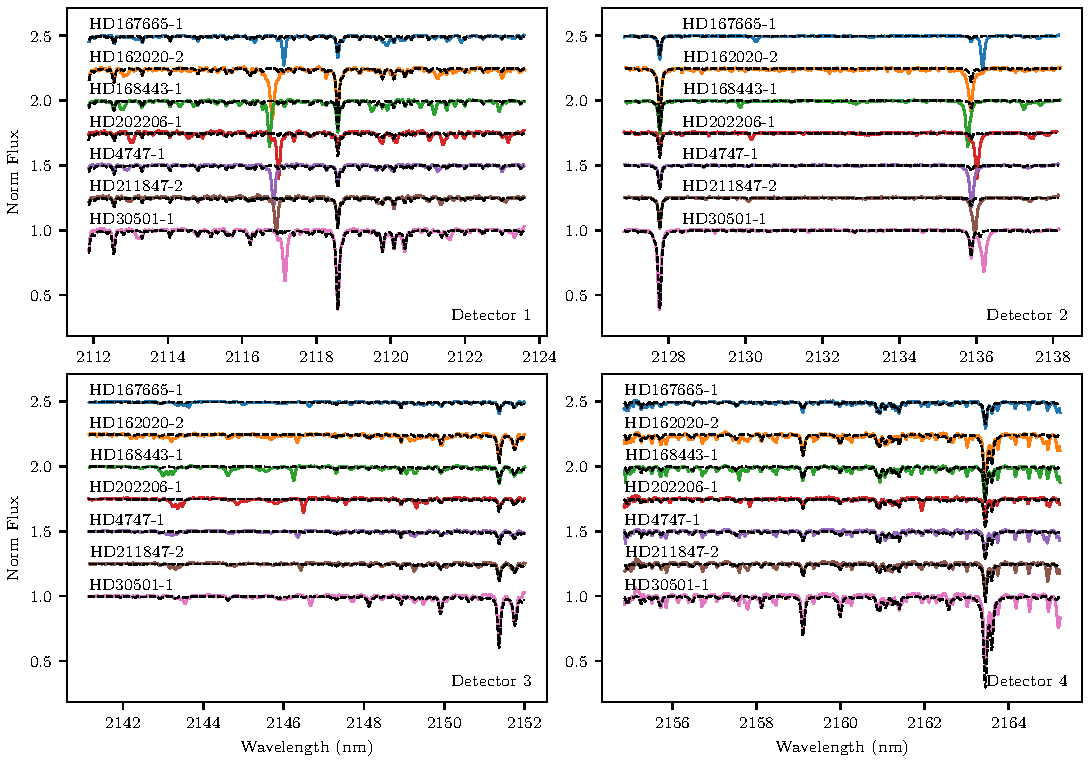
\includegraphics[width=\hsize]{figures/reduction/Spectra_examples.pdf}
% 	\caption{Extracted, normalized and wavelength calibrated spectra for a single observation of each target. The target name is given above each spectrum along with the observation number. Each panel is the spectra from a single detector 1--4 in order of increasing wavelength. The black dashed lines indicate the unique telluric spectrum used for wavelength calibration and telluric correction for each observation.}
% 	\label{fig:detector4allspectra}
% \end{figure*}



\unfinished{See Solene's paper regarding Telluric correction with models and reference spectra}

Telluric Correction:
TAPAS
Requiring data from tapas
- not handy for many
- own script to derive from spectra header.

\unfinished{Artigau 2018 use TAPAS, and Figueria 2016}

\subsubsection{Telluric correction}
\label{subsec:telluric_correction}
Ground based observations require the removal of the absorption lines introduced by Earth's atmosphere. These observations were first taken in an atmospheric window of the K-band in order to reduce the absorption introduced by the atmosphere \citep{barnes_hd_2008}. To correct for the remaining telluric line contamination the spectra were divided by the TAPAS\citep{bertaux_tapas_2014} atmospheric transmission models for each observation. Synthetic telluric models were used to avoid the observing overhead necessary to perform telluric standard star exposures \citep{vacca_method_2003}, and they have been demonstrated to be superior in the quality of the correction relative to the telluric standard approach \citep[e.g.][]{cotton_atmospheric_2014}.

Before the correction, the depth of the telluric lines were re-scaled to match the airmass of the observation using the relation \(\rm T = T^{\beta} \), where \(\rm T\) is the telluric spectrum and \(\beta \) is the airmass ratio between the observation and model. This changed the depth of most absorption lines to match the observations, but does not correctly scale the deeper \(\rm H_{2}O \) lines. The scaled telluric model is interpolated to the wavelengths of the observed spectrum and then used to correct the observed spectra through division, leaving behind a telluric corrected spectra. An example of a telluric corrected spectra is shown in the middle panel of Fig.~\ref{fig:spectral_example}, with the light blue shading indicating where the deeper telluric lines were.

We attempted the technique suggested by \citet{bertaux_tapas_2014} to address the poor \(\rm H_{2}O \) airmass scaling, to fit a scaling factor to the \(\rm {H}_{2}O \) absorption lines before convolution to the instrument resolution. This was achieved by first dividing the spectrum by a telluric model with only non-\(\rm H_{2}O \) constituents, convolved to the observed resolution, and scaled by the airmass to remove the non-\(\rm H_{2}O \) lines. Then a model with only \(\rm H_{2}O \) lines at full resolution was scaled by a factor \(\textrm{T}^{x} \), convolved to \(\rm R=50\,000 \) and compared to the observed spectra. The factor \(x \) was fitted to find the best scaling factor for the \(\rm H_{2}O \) lines.

We found that for a few spectra in our sample this method corrected the deeper telluric lines well, but in many cases we found that the fitted scaling factor was affected by the presence of blended stellar lines (attempting to fit those also). It was also strongly influenced by the deepest \(H_{2}O\) telluric lines present. We find that the telluric correction of the deep \(\rm H_{2}O \) lines could be improved with this technique, but, at the cost of worsening the correction of the many smaller \(\rm H_{2}O \) lines. Since the smaller \(\rm H_{2}O \) lines covered more of the spectrum in this region than the larger lines we chose not to continue with this separate \(\rm H_{2}O \) scaling. One possible solution for this would be to perform a piece-wise telluric correction, performing this step only for the deeper \( \rm H_{2}O\) lines, or by using one of the other tools that fits the telluric model to the observations. This technique could also benefit from a larger wavelength span that would enable blended lines to be ignored while having sufficient deep \(\rm H_{2}O\) lines to fit the scaling factor correctly. This small experiment shows that a simple scaling is not enough to correct for the absorption in an effective way, for this case.

\unfinished{Add telluric spectra for NIR band? the plot from Molecfit?}

\unfinished{Still uneven line coverage on all detectors in this small range}


\subsection{Tapas models}
\label{subsec:tapas_models}
We used telluric line models to wavelength calibrate the reduced spectra in Sect.~\ref{subsec:wave_cal} and to correct for the atmospheric absorption in Sect.~\ref{subsec:telluric_correction}. We utilized the TAPAS (Transmissions of the AtmosPhere for AStronomical data) web-service\footnote{\url{http://www.pole-ether.fr/tapas/}} \citep{bertaux_tapas_2014} to obtain atmospheric transmission models for each observation. TAPAS uses the standard line-by-line radiation transfer model code LBLRTM~\citep{clough_linebyline_1995} along with the 2008 HITRAN spectroscopic database~\citep{rothman_hitran_2009} and Arletty atmospheric profiles derived using meteorological measurements from the ETHER data center\footnote{\url{http://www.pole-ether.fr}}, which has a 6 hour resolution in atmospheric profiles.
We use the mid-observation time to retrieve transmission models for each observation, with the Arletty atmospheric profiles\footnote{Nearest of the 6 hourly profiles} and vacuum wavelengths. The telluric models were retrieved without any barycentric correction to keep the telluric lines at a RV of zero with respect to the instrument. We obtained one model with all provided species present, convolved to a resolution of \(\rm R=50\,000 \), and another two models without an instrumental profile convolution applied. For these two extra models, one contained only the transmission spectra of \(\rm H_{2}O \) while the other was for all other constituents except \(\rm H_{2}O \). This was to explore a known issue \citep{bertaux_tapas_2014} with the depth of \(\rm H_{2}O \) absorption lines in Sect.~\ref{subsec:telluric_correction}.

After the telluric correction is performed, the spectra are corrected for Earth's barycentric RV using the \emph{helcor} PyAstronomy\footnote{https://pyastronomy.readthedocs.io} function ported from the REDUCE IDL package (See \citet[][]{piskunov_new_2002}).


\subsection{Wavelength masking}
We apply several wavelength masks to remove wavelength regions from which we cannot extract information.
Firstly, regions near the edges of each detector where the wavelength solution is extrapolated outside of the calibrating telluric lines are removed, reducing the effective size of each detector by about \(10\%\) or \(\sim100\) pixels. 

Secondly, we mask out any remaining artifacts present in the spectra and the centers of deep telluric lines where telluric correction was not corrected properly, sometimes resulting in "emission-like" peaks in the corrected spectrum. These factors combined result in masking out around a further 10\% of the observed spectra. 

In Sect.~\ref{sec:results} we also apply a further wavelength restriction to mask out regions where there is a large mismatch between the observed spectrum and the closest synthetic spectra to the host. This significantly restricts the wavelength span utilized for that purpose to around only 43\% and the masked regions are visible in Fig.~\ref{fig:visualinspection-hd2118471}. 


\unfinished{ADD non/H20 fitting corrections.}

\missingfigure{Plots showing some examples the telluric correction with and without H20 separated}

\section{Reduction experience:}
The effort placed in reducing CRIRES spectra allowed me to participate in 3 different collaborations.

I was asked to reduce the CRIRES observations of xxxx to try and derive spectroscopic parameters in the NIR. Unfortunately this was never used and they decided to use Barnard's Star from the CRIRES-POP library instead.

I reduced the spectra of $\eta$ Tau a rotating brown dwarf at the request of a collaborator outside of Portugal.
  
eta TAU - Rotating brown dwarf. This will hopefully result in a publication, (XXX in prep.?)

The reduced spectra of eta TAU were also used by a college to assess the effectiveness of different telluric correction methods resulting in a publication \citet{Ulmer-moll_2018}.
